% =====================================================================
%  Exercise 2: Barrier Synchronization
%  Author: Nguyen Le Hoang Hung (2570214)
%  Source code: ex2_barrier/ (barriers.hpp, test_barrier.cpp,
%               bench_barrier.cpp, plot_results.py, build.sh)
%  Requires in the preamble: pgfplots (\pgfplotsset{compat=1.18}),
%  algorithm2e, listings, booktabs, siunitx, amsthm, graphicx.
% =====================================================================

\section{Barrier Synchronization}
\label{sec:ex2}

\subsection{Problem Statement and Objectives}
\label{sec:ex2-objectives}

A \emph{barrier} is a synchronization point for a fixed group of $N$ threads:
no thread may pass the barrier until all $N$ threads have reached it. The
assignment asks us to:

\begin{enumerate}
    \item implement the \textbf{Sense-Reversing Barrier} discussed in the
          lecture for multi-threaded C++ programs;
    \item devise an approach for \textbf{testing the correctness} of the
          implementation;
    \item conduct a \textbf{performance and scalability study} on every
          shared-memory platform available to the group, using
          \emph{the number of completed barrier episodes per unit time with
          no useful work between barriers} as the metric, and compare the
          implementation with existing barriers (OpenMP, Pthreads, C++);
    \item optionally, evaluate \textbf{exponential backoff} as a way to
          reduce contention.
\end{enumerate}

Our deliverables for this exercise are summarised below. All source code is
in the directory \texttt{ex2\_barrier/} of the submission.

\begin{table}[H]
\centering
\caption{Source files of Exercise 2.}
\label{tab:ex2-files}
\begin{tabular}{l p{11.6cm}}
\toprule
\textbf{File} & \textbf{Content} \\
\midrule
\texttt{barriers.hpp}       & The sense-reversing barrier (three waiting policies, two
                              memory orderings), wrappers around \texttt{std::barrier}
                              and \texttt{pthread\_barrier\_t}, and the two broken
                              barriers from the lecture, used for mutation testing. \\
\texttt{test\_barrier.cpp}  & Correctness test harness: invariant checks, random
                              delays, a hang watchdog, and a \texttt{-{}-buggy} mode. \\
\texttt{bench\_barrier.cpp} & Throughput benchmark (episodes per second) for all
                              barriers including \texttt{\#pragma omp barrier};
                              writes CSV. \\
\texttt{cli.hpp}            & Command-line helpers shared by the two programs. \\
\texttt{plot\_results.py}   & Plots benchmark CSV files. \\
\texttt{build.sh}           & Build script (GCC/Clang, C++20); detects OpenMP support. \\
\texttt{run\_all.sh}        & Runs the complete study on one machine: build, system
                              information, tests, benchmarks; packs the results. \\
\bottomrule
\end{tabular}
\end{table}

% ---------------------------------------------------------------------
\subsection{Background}
\label{sec:ex2-background}

\subsubsection{Semantics of a barrier}

Barriers separate the \emph{computational phases} of a parallel program,
e.g.\ initialisation, the iterations of a numerical solver, and output. Each
use of the barrier by all $N$ threads is called an \emph{episode}. An
implementation consists of two phases~\cite{lecture04,scott2013}:

\begin{itemize}
    \item \textbf{Arrival phase}: a thread announces that it has reached the
          barrier.
    \item \textbf{Departure (waiting) phase}: a thread waits until it knows
          that all other threads have arrived, then leaves.
\end{itemize}

Waiting can be done by \emph{busy-waiting} (spinning on a memory location)
or by \emph{scheduler-based} blocking (the thread sleeps in the kernel and
is woken up). The sense-reversing barrier is a busy-waiting barrier.

A barrier must satisfy three properties:

\begin{description}
    \item[Safety] No thread leaves episode $e$ before all $N$ threads have
          arrived at episode $e$.
    \item[Liveness] Once all $N$ threads have arrived, every thread
          eventually leaves.
    \item[Reusability] The same barrier object can be used for an unbounded
          sequence of episodes, even when fast threads arrive at episode
          $e+1$ while slow threads are still leaving episode $e$.
\end{description}

\subsubsection{Memory ordering requirements}

Programs use barriers to exchange data between phases: values written by
any thread \emph{before} the barrier must be visible to every thread
\emph{after} it. Using the reordering notation of the
lecture~\cite{lecture04}:

\begin{itemize}
    \item operations before the barrier must not be reordered after the
          arrival, so the arrival needs an \textbf{RW$\|$} (release)
          restriction;
    \item operations after the barrier must not be reordered before the
          departure, so the departure needs a \textbf{$\|$RW} (acquire)
          restriction.
\end{itemize}

Taken together, a barrier acts as a full \textbf{RW$\|$RW} fence across the
whole group of threads. In C++ this maps onto
\texttt{memory\_order\_release} for the writes that signal arrival or
release, and \texttt{memory\_order\_acquire} for the reads that observe
them~\cite{cppmemorder}.

\subsubsection{Why the naive centralized barrier fails}
\label{sec:ex2-naive}

The lecture builds up to the sense-reversing barrier through two broken
attempts. We implemented both (Listing~\ref{lst:ex2-buggy}) because they
also serve as ``known-bad'' inputs for our test harness
(Section~\ref{sec:ex2-mutation}).

\begin{lstlisting}[caption={The two broken centralized barriers from the lecture (simplified from \texttt{barriers.hpp}).},label={lst:ex2-buggy}]
// Attempt 1 (lecture 04, slide 10): spin on the counter itself.
void BuggyCountBarrier::arrive_and_wait(int) {
    if (count_.fetch_add(1) == n_ - 1) {
        count_.store(0);                         // reset for next episode
    } else {
        while (count_.load() != n_ - 1) cpu_relax();   // spin
    }
}

// Attempt 2 (lecture 04, slide 12): spin on a separate flag.
void BuggyFlagBarrier::arrive_and_wait(int) {
    if (count_.fetch_add(1) == n_ - 1) {
        count_.store(0);
        wait_.store(false);                      // release everyone
    } else {
        while (wait_.load()) cpu_relax();        // spin
    }
    // There is no safe moment to set wait_ back to true.
}
\end{lstlisting}

\paragraph{Attempt 1 (spin on the counter).} The last thread resets
\texttt{count} to $0$ immediately after incrementing it to $N$. A waiting
thread that does not read \texttt{count} during the short window in which
it equals $N-1$ never sees the triggering value and \textbf{spins forever}.
This is a liveness violation. The attempt has a second, less obvious
flaw: the thread that arrives \emph{second to last} raises \texttt{count}
to $N-1$ itself, so its own spin condition is satisfied immediately and it
\textbf{leaves before the last thread has arrived}. This is a safety
violation. Our tests revealed this second bug
(Section~\ref{sec:ex2-correct-results}).

\paragraph{Attempt 2 (spin on a flag).} Waiting on a separate flag fixes the
lost-wake-up problem, but the flag must be re-armed (set back to
\texttt{true}) before the next episode. The last arriver cannot do this
safely: it does not know when every waiter has observed \texttt{false}, and
a fast thread may already have re-entered the barrier for the next episode.
If the flag is never re-armed, every episode after the first lets threads
pass \textbf{without waiting}. This is a safety violation. A plain counter is
enough for a \emph{one-time} barrier (a \emph{latch}, \texttt{std::latch} in
C++20) but not for a reusable one.

% ---------------------------------------------------------------------
\subsection{The Sense-Reversing Barrier}
\label{sec:ex2-algorithm}

\subsubsection{Idea}

Instead of resetting the flag, the sense-reversing barrier \emph{inverts the
meaning} of the flag in every episode~\cite{lecture04,herlihy2012,mcs1991}.
The shared Boolean \texttt{sense} alternates between \texttt{true} and
\texttt{false} from one episode to the next, and each thread keeps a private
copy \texttt{local\_sense} of the value it expects for the \emph{current}
episode. Because consecutive episodes wait for \emph{opposite} values of
\texttt{sense}, a thread that is still leaving episode $e$ and a thread that
has already arrived at episode $e+1$ can never be confused.

\begin{algorithm}[H]
\caption{Sense-reversing barrier (lecture 04, slide 14)}
\label{alg:ex2-srb}
\SetKwProg{Fn}{procedure}{}{end}
\SetKw{KwShared}{shared}
\SetKw{KwLocal}{thread-local}
\KwShared \texttt{count} $\gets 0$\tcp*{number of threads arrived}
\KwShared \texttt{sense} $\gets$ \texttt{true}\tcp*{global sense}
\KwLocal \texttt{local\_sense}$[i] \gets$ \texttt{true} for every thread $i$\;
\BlankLine
\Fn{\texttt{arrive\_and\_wait}$(i)$}{
    \texttt{local\_sense}$[i] \gets \lnot$\,\texttt{local\_sense}$[i]$\tcp*{expected value for this episode}
    \tcp{arrival: fetch-and-increment with RW$\|$ ordering}
    \eIf{\textup{FAI}$(\texttt{count}) = N-1$}{
        \texttt{count} $\gets 0$\tcp*{re-arm for the next episode}
        \texttt{sense} $\gets$ \texttt{local\_sense}$[i]$\tcp*{release all waiters, RW$\|$}
    }{
        \While{\texttt{sense} $\neq$ \texttt{local\_sense}$[i]$}{
            spin\tcp*{departure, $\|$RW}
        }
    }
}
\end{algorithm}

\subsubsection{Walk-through}

Table~\ref{tab:ex2-trace} traces two consecutive episodes with $N=3$ threads
$T_0,T_1,T_2$. Note how $T_2$, the last thread of episode~1, releases the
others by setting \texttt{sense} to \texttt{false}. In episode~2, $T_0$ (the
fastest thread) re-enters while $T_1$ has not even observed the release
yet. This is harmless: $T_0$ now waits for \texttt{sense = true}, a value
that will only be written by the last arriver of episode~2.

\begin{table}[H]
\centering
\caption{Execution trace of Algorithm~\ref{alg:ex2-srb} with $N=3$
(\texttt{ls}$_i$ = \texttt{local\_sense}$[i]$, T = \texttt{true}, F =
\texttt{false}).}
\label{tab:ex2-trace}
\small
\begin{tabular}{r p{4.4cm} c c c c c p{3.9cm}}
\toprule
Step & Event & \texttt{count} & \texttt{sense} & \texttt{ls}$_0$ & \texttt{ls}$_1$ & \texttt{ls}$_2$ & Comment \\
\midrule
0  & initial state                    & 0 & T & T & T & T & \\
1  & $T_0$ arrives (FAI returns 0)    & 1 & T & F & T & T & $T_0$ spins until \texttt{sense}=F \\
2  & $T_1$ arrives (FAI returns 1)    & 2 & T & F & F & T & $T_1$ spins until \texttt{sense}=F \\
3  & $T_2$ arrives (FAI returns 2)    & 3 & T & F & F & F & $T_2$ is the last arriver \\
4  & $T_2$ resets \texttt{count}      & 0 & T & F & F & F & \\
5  & $T_2$ writes \texttt{sense}=F    & 0 & F & F & F & F & episode 1 complete \\
6  & $T_0$ sees F, leaves; $T_2$ leaves & 0 & F & F & F & F & $T_1$ has not looked yet \\
7  & $T_0$ arrives at episode 2       & 1 & F & T & F & F & $T_0$ spins until \texttt{sense}=T \\
8  & $T_1$ finally sees F, leaves     & 1 & F & T & F & F & not confused by $T_0$ \\
9  & $T_1$, $T_2$ arrive at episode 2 & 3 & F & T & T & T & last arriver resets, writes T \\
\bottomrule
\end{tabular}
\end{table}

\subsubsection{Correctness argument}
\label{sec:ex2-proof}

Let $s_e$ denote the value of \texttt{sense} at the end of episode $e$
($s_0 = $ \texttt{true}). Then $s_e = s_{e-1}$ negated, and in episode $e$
every thread expects \texttt{local\_sense}$ = s_e$.

\begin{lemma}[Safety]
No thread leaves episode $e$ before all $N$ threads have arrived at
episode $e$.
\end{lemma}
\begin{proof}
A thread leaves either as the last arriver, whose fetch-and-increment
returned $N-1$, or by observing \texttt{sense} $= s_e$. Within episode $e$,
\texttt{count} starts at $0$ (it was reset by the previous last arriver, see
the next lemma), so FAI returns $N-1$ only to the $N$-th arriving thread.
The value $s_e$ is written to \texttt{sense} only by that thread, after its
FAI. Before that write, \texttt{sense} holds $s_{e-1} \neq s_e$. Hence no
waiter can observe $s_e$ before all $N$ threads have performed their FAI,
i.e.\ arrived.
\end{proof}

\begin{lemma}[Reusability]
Threads in episode $e+1$ cannot interfere with threads still leaving
episode $e$.
\end{lemma}
\begin{proof}
A thread can enter episode $e+1$ only after leaving episode $e$, i.e.\ after
the last arriver of episode $e$ has executed \texttt{count} $\gets 0$
followed by \texttt{sense} $\gets s_e$. Hence its FAI in episode $e+1$ is
applied to the reset counter. While some threads are still leaving episode
$e$, \texttt{sense} keeps the value $s_e$ until the last arriver of episode
$e+1$ writes $s_{e+1}$. That cannot happen before \emph{every} thread,
including the slow ones, has arrived at episode $e+1$, and hence has already
left episode $e$. Slow threads therefore always see $s_e$ when they look,
and early threads of episode $e+1$ wait for $s_{e+1}$.
\end{proof}

\begin{lemma}[Liveness]
If all $N$ threads arrive at episode $e$, all of them eventually leave.
\end{lemma}
\begin{proof}
The $N$-th FAI returns $N-1$, so the last arriver leaves without waiting and
writes $s_e$. By the previous lemma, \texttt{sense} keeps the value $s_e$
until every thread has left episode $e$. By cache coherence, every spinning
thread eventually reads $s_e$. Unlike Attempt~1, the value it waits for is
not overwritten too early.
\end{proof}

\begin{proposition}[Memory visibility]
With the memory orderings of Section~\ref{sec:ex2-orders}, every write
performed by any thread before episode $e$ \emph{happens-before} every
operation performed by any thread after episode $e$.
\end{proposition}
\begin{proof}
Let $T_j$ be any thread and $T_\ell$ the last arriver.
(i)~$T_j$'s earlier writes are sequenced before its FAI (a release RMW).
$T_\ell$'s FAI (an acquire RMW) reads a value in the release sequence headed
by $T_j$'s FAI, because the intermediate RMWs of other threads extend
release sequences. Therefore $T_j$'s FAI synchronizes-with $T_\ell$'s FAI.
(ii)~$T_\ell$'s store to \texttt{sense} is a release, and a waiter $T_k$
reads it with an acquire load, so the store synchronizes-with that load.
Chaining (i), sequencing within $T_\ell$, and (ii) gives
$\text{write}_j \rightarrow_{hb} \text{FAI}_j \rightarrow_{hb}
\text{FAI}_\ell \rightarrow_{hb} \text{store}_\ell \rightarrow_{hb}
\text{load}_k \rightarrow_{hb} \text{any later operation of } T_k$.
For $T_k = T_\ell$, step (ii) is unnecessary.
\end{proof}

\subsubsection{Cost model}
\label{sec:ex2-costmodel}

Per episode, the barrier performs $N$ atomic RMW operations on the same
memory location (\texttt{count}), one plain store to \texttt{count}, one
store to \texttt{sense}, and the spinning reads. On a cache-coherent
machine:

\begin{itemize}
    \item \textbf{Spinning is cheap.} While waiting, each thread reads its
          own cached copy of \texttt{sense} (cache line in \emph{Shared}
          state), which generates no interconnect traffic. The single
          release store invalidates all copies, and each waiter then incurs
          one cache miss to fetch the new value~\cite{lecture04,sorin2020}.
    \item \textbf{Arrival is the bottleneck.} Each FAI needs the cache line
          of \texttt{count} in the \emph{Modified} (exclusive) state. The
          $N$ FAIs are therefore serialized, and the line migrates between
          cores up to $N$ times per episode. We expect the time per episode
          to grow roughly \emph{linearly} in $N$, i.e.\
          $T_{\text{episode}}(N) \approx N \cdot t_{\text{transfer}}$, where
          $t_{\text{transfer}}$ is the cost of moving one cache line between
          cores.
\end{itemize}

The lecture names two remedies for large machines: tree-structured
barriers (combining tree and static tree), which spread the counter over
many cache lines, and the dissemination barrier, which avoids RMW operations
altogether and completes in $\lceil \log_2 N\rceil$ rounds. They are outside
the scope of this exercise, but they help explain our scalability results.

% ---------------------------------------------------------------------
\subsection{Implementation in C++}
\label{sec:ex2-impl}

\subsubsection{Design overview}

All barriers implement the same minimal interface, which allows the test
harness and the benchmark to be written once, as templates:

\begin{lstlisting}[numbers=none]
explicit Barrier(int num_threads);
void arrive_and_wait(int tid);      // tid in [0, num_threads)
\end{lstlisting}

The thread id \texttt{tid} indexes the thread-local sense array, exactly as
\texttt{lsense[self]} on the lecture slide. Library barriers ignore it.
The sense-reversing barrier is a class template with two compile-time
parameters, so every variant is compiled to specialised code without any
run-time dispatch in the hot loop:

\begin{itemize}
    \item \texttt{Wait}: the waiting policy, i.e.\ what a thread does in each
          iteration of the spin loop (Section~\ref{sec:ex2-wait});
    \item \texttt{Order}: the memory orderings used for the atomic
          operations (Section~\ref{sec:ex2-orders}).
\end{itemize}

\subsubsection{Core implementation}

Listing~\ref{lst:ex2-srb} shows the barrier as implemented in
\texttt{barriers.hpp} (comments shortened).

\begin{lstlisting}[caption={Sense-reversing barrier (\texttt{barriers.hpp}).},label={lst:ex2-srb}]
inline constexpr std::size_t kCacheLine = 128;

template <class Wait = SpinWait, Order O = Order::AcqRel>
class SenseReversingBarrier {
public:
    explicit SenseReversingBarrier(int num_threads)
        : n_(num_threads), local_(static_cast<std::size_t>(num_threads)) {}

    void arrive_and_wait(int tid) {
        // Flip this thread's sense: consecutive episodes wait for
        // opposite values of the shared flag.
        const bool my_sense = !local_[tid].sense;
        local_[tid].sense = my_sense;

        // Arrival: release publishes our earlier writes (RW||),
        // acquire lets the last arriver see everyone else's writes.
        if (count_.fetch_add(1, kRmw) == n_ - 1) {
            count_.store(0, kReset);              // re-arm the counter
            sense_.store(my_sense, kRelease);     // release all waiters
        } else {
            Wait w;                               // fresh policy state
            while (sense_.load(kAcquire) != my_sense) w.pause();  // ||RW
        }
    }

private:
    // kRmw = acq_rel, kRelease = release, kAcquire = acquire,
    // kReset = relaxed   (all seq_cst for Order::SeqCst)
    struct alignas(kCacheLine) LocalSense { bool sense = true; };

    const int n_;
    alignas(kCacheLine) std::atomic<int>  count_{0};
    alignas(kCacheLine) std::atomic<bool> sense_{true};
    std::vector<LocalSense> local_;       // one padded slot per thread
};
\end{lstlisting}

\subsubsection{Choice of memory orderings}
\label{sec:ex2-orders}

Table~\ref{tab:ex2-orders} maps the reordering restrictions of the lecture
pseudocode to the C++ memory orders we use. The default variant
(\texttt{Order::AcqRel}) uses the weakest orderings for which the proof in
Section~\ref{sec:ex2-proof} holds.

\begin{table}[H]
\centering
\caption{Memory orderings in the sense-reversing barrier.}
\label{tab:ex2-orders}
\small
\begin{tabular}{p{3.7cm} p{2.0cm} p{1.7cm} p{6.6cm}}
\toprule
\textbf{Operation} & \textbf{Lecture} & \textbf{C++ order} & \textbf{Reason} \\
\midrule
\texttt{count.fetch\_add(1)} & FAI(RW$\|$) & \texttt{acq\_rel} &
  \emph{Release}: publishes the arriving thread's writes. \emph{Acquire}:
  needed by the last arriver, which leaves without reading \texttt{sense}
  and must see all other threads' writes. \\
\texttt{count.store(0)} & --- & \texttt{relaxed} &
  Re-entering threads synchronize through the release store to
  \texttt{sense}, which is sequenced after this reset, so they always
  observe $0$. \\
\texttt{sense.store(s)} & RW$\|$ & \texttt{release} &
  Publishes everything the last arriver has seen, including (transitively)
  the writes of all other threads. \\
\texttt{sense.load()} (spin) & fence(R$\|$RW) & \texttt{acquire} &
  Prevents operations after the barrier from moving before the departure. \\
\bottomrule
\end{tabular}
\end{table}

For comparison we also built two other orderings:

\begin{itemize}
    \item \texttt{sense-seqcst}: all operations use
          \texttt{memory\_order\_seq\_cst} (the C++ default). This is
          correct, but may cost more. On x86, a sequentially consistent
          \emph{store} is compiled to an \texttt{XCHG} instruction (an
          implicitly locked full fence), while a release store is a plain
          \texttt{MOV}.
    \item \texttt{sense-relaxed}: all operations use
          \texttt{memory\_order\_relaxed}. This is \textbf{incorrect by the
          C++ memory model}: it gives no happens-before relation, so data
          written before the barrier is not guaranteed to be visible after
          it. We keep it only as a mutation for testing
          (Section~\ref{sec:ex2-mutation}).
\end{itemize}

\subsubsection{Avoiding false sharing}

All hot variables are aligned to separate cache lines
(\texttt{alignas(128)}):

\begin{itemize}
    \item \texttt{count\_} and \texttt{sense\_} live on \emph{different}
          lines. If they shared a line, every arriving thread's FAI would
          invalidate the waiters' cached copy of \texttt{sense\_}, and
          spinning would no longer be ``free''.
    \item Each thread's \texttt{local\_sense} is padded to its own line, so
          writing one's own sense never invalidates another thread's line.
\end{itemize}

We pad to 128 bytes rather than the 64-byte line size of x86 because Intel
processors prefetch cache lines in adjacent pairs (the spatial prefetcher),
and Apple M-series processors use 128-byte lines. The memory overhead is
negligible.

\subsubsection{Waiting policies and exponential backoff}
\label{sec:ex2-wait}

The spin loop calls \texttt{w.pause()} after each unsuccessful check. A new
policy object is created for every wait, so any backoff state starts fresh
in every episode. We implemented three policies
(Listing~\ref{lst:ex2-wait}):

\begin{description}
    \item[\texttt{SpinWait} (\texttt{sense-spin})] executes a single
          \texttt{PAUSE} instruction (\texttt{\_mm\_pause()} on x86,
          \texttt{yield} on ARM). \texttt{PAUSE} tells the core it is in a
          spin loop: it saves power, frees resources for the sibling
          hyper-thread, and avoids the memory-order mis-speculation penalty
          when the loop exits~\cite{intelopt}.
    \item[\texttt{BackoffWait} (\texttt{sense-backoff})] performs
          \emph{exponential backoff}: after the $k$-th failed check it
          pauses $\min(2^{k}, 1024)$ times. This is the technique suggested
          in the assignment for reducing contention.
    \item[\texttt{YieldWait} (\texttt{sense-yield})] spins for 128
          iterations, then calls \texttt{std::this\_thread::yield()} in each
          further iteration, giving the core back to the OS scheduler. This
          follows the ``spin for a while, then yield'' strategy of the
          lecture, and is meant for runs with more threads than cores.
\end{description}

\begin{lstlisting}[caption={Waiting policies (\texttt{barriers.hpp}).},label={lst:ex2-wait}]
struct SpinWait {
    void pause() { cpu_relax(); }                    // _mm_pause()
};

template <unsigned MaxSpins = 1024>
struct BackoffWaitT {                                // exponential backoff
    unsigned limit = 1;
    void pause() {
        spin_for(limit);                             // `limit` PAUSEs
        if (limit < MaxSpins) limit <<= 1;           // double, up to the cap
    }
};

template <unsigned SpinsBeforeYield = 128>
struct YieldWaitT {                                  // spin, then yield
    unsigned spins = 0;
    void pause() {
        if (spins < SpinsBeforeYield) { ++spins; cpu_relax(); }
        else std::this_thread::yield();
    }
};
\end{lstlisting}

\subsubsection{Barriers used for comparison}

\begin{description}
    \item[\texttt{std-barrier}] C++20 \texttt{std::barrier<>}~\cite{cppbarrier},
          a reusable barrier from the standard library. In GCC's libstdc++
          it is built on \texttt{std::atomic::wait/notify}, which spins
          briefly and then blocks.
    \item[\texttt{pthread-barrier}] POSIX \texttt{pthread\_barrier\_t}
          (provided on Windows by \texttt{winpthreads}), which blocks
          threads using a mutex and condition variables.
    \item[\texttt{openmp}] \texttt{\#pragma omp barrier} inside an
          \texttt{omp parallel} region (GNU libgomp). It is not an object,
          so it has its own timing routine (Listing~\ref{lst:ex2-bench}).
          Its waiting behaviour is controlled by the
          \texttt{OMP\_WAIT\_POLICY} environment variable
          (\texttt{active} = spin, \texttt{passive} = sleep)~\cite{openmp52}.
\end{description}

% ---------------------------------------------------------------------
\subsection{Correctness Testing Methodology}
\label{sec:ex2-testing}

Testing cannot prove a concurrent algorithm correct; that is the role of
the argument in Section~\ref{sec:ex2-proof}. A good test, however, must
(a)~check exactly the properties a barrier promises, (b)~exercise many
different interleavings, and (c)~be shown to detect real bugs. Our harness
\texttt{test\_barrier} is designed around these three goals.

\subsubsection{Invariants checked after every episode}

Each of the $N$ threads executes $E$ episodes (default
$E = \num{100000}$). Listing~\ref{lst:ex2-test} shows the per-thread loop.
In episode $e$, thread $i$:

\begin{enumerate}
    \item optionally waits for a random time (with probability $1/16$, a
          spin of $0$--$1999$ \texttt{PAUSE}s), so that threads arrive in a
          different order in different episodes;
    \item writes $e$ into its own slot \texttt{slot}$[i]$ and increments a
          shared counter \texttt{arrivals};
    \item calls \texttt{arrive\_and\_wait}$(i)$;
    \item checks three invariants:
\end{enumerate}

\begin{description}
    \item[(I1) Visibility] $\forall j:\ \texttt{slot}[j] = e$. Every thread
          has written its slot before the barrier, and all those writes are
          visible after it. A failure means a thread left too early
          \emph{or} the barrier lacks the required memory ordering.
    \item[(I2) No early departure] $\texttt{arrivals} \geq (e+1)\,N$. All
          $N$ arrivals of episodes $0..e$ have happened.
    \item[(I3) No overtaking] $\texttt{arrivals} \leq (e+2)\,N - 1$. At most
          the $N-1$ \emph{other} threads can already have arrived at episode
          $e+1$. If the value is larger, some thread has passed the
          \emph{next} barrier without waiting for us.
\end{description}

\begin{lstlisting}[caption={Per-thread test loop (\texttt{test\_barrier.cpp}, simplified).},label={lst:ex2-test}]
for (long e = 0; e < episodes; ++e) {
    Slot* cur = buf[e & 1].get();                 // double buffering
    if (delays && (rng() & 15) == 0) spin_for(rng() % 2000);

    cur[tid].v.store(e, relaxed);                 // publish "I am in episode e"
    arrivals.fetch_add(1, relaxed);

    barrier.arrive_and_wait(tid);

    for (int j = 0; j < n; ++j)                   // (I1) visibility
        if (cur[j].v.load(relaxed) != e) report(...);
    long a = arrivals.load(relaxed);
    if (a < (e + 1) * n)     report(...);         // (I2) no early departure
    if (a > (e + 2) * n - 1) report(...);         // (I3) no overtaking
}
\end{lstlisting}

\paragraph{Why the checks have no false positives.} Two design details make
the invariants hold \emph{exactly} for any correct barrier:

\begin{itemize}
    \item \textbf{Double buffering.} Slots for even and odd episodes live in
          two separate arrays. A fast thread writing episode $e+1$ uses the
          other array. It could only overwrite a slot that someone is still
          checking for episode $e$ when it writes episode $e+2$, and it can
          start episode $e+2$ only after every thread, including the
          checker, has arrived at the barrier of episode $e+1$, i.e.\ after
          the checker has finished its checks.
    \item \textbf{Relaxed atomics for test data.} The slots and the counter
          are atomics accessed with \texttt{memory\_order\_relaxed}. This
          keeps the program free of undefined behaviour even when a broken
          barrier is tested (no data race on plain variables). It also
          means the test adds no synchronization of its own: the
          \emph{only} source of happens-before ordering between the write
          and the check is the barrier itself, so (I1) really tests the
          barrier's memory ordering.
\end{itemize}

\subsubsection{Exercising many interleavings}

\begin{itemize}
    \item \textbf{Thread counts.} $N \in \{2, 3, 4, H, 2H\}$ with $H$ the
          number of hardware threads: small counts, a non-power of two
          ($N=3$), one thread per hardware thread, and
          \emph{oversubscription} ($2H$ threads), where threads are
          preempted by the OS in the middle of an episode.
    \item \textbf{Random delays} change the arrival order and the identity
          of the last arriver from episode to episode, and create situations
          where some threads are far ahead of others, which is exactly the
          case that breaks Attempt~2.
    \item \textbf{Many episodes} ($10^5$ per configuration, $3000$ when
          oversubscribed, $300$ for pure spinning when oversubscribed)
          make rare interleavings likely to appear.
\end{itemize}

\subsubsection{Hang detection}

Liveness bugs (such as Attempt~1) manifest as hangs, not as wrong values. A
watchdog in the main thread samples the \texttt{arrivals} counter every
\SI{5}{\milli\second}. If the counter does not change for a timeout period
(\SI{120}{\second} by default, \SI{10}{\second} in \texttt{--buggy} mode),
it reports a \textbf{HANG} together with the episode in which the threads
are stuck. A hung thread cannot be stopped or joined, so the program then
exits.

\subsubsection{Mutation testing: does the test catch real bugs?}
\label{sec:ex2-mutation}

A test that never fails is only convincing if it is shown to fail on broken
code. The option \texttt{--buggy} runs the harness on three deliberately
broken barriers:

\begin{enumerate}
    \item \texttt{buggy-flag}: Attempt~2 (flag never re-armed), expected to
          violate (I1)--(I3);
    \item \texttt{sense-relaxed}: the correct algorithm without memory
          ordering, expected to violate (I1) on hardware with a weak memory
          model;
    \item \texttt{buggy-count}: Attempt~1 (spin on the counter), expected to
          hang, and to let the second-to-last thread leave early.
\end{enumerate}

% ---------------------------------------------------------------------
\subsection{Experimental Setup}
\label{sec:ex2-setup}

\subsubsection{Platforms}

\begin{table}[H]
\centering
\caption{Shared-memory platforms used in the experiments.}
\label{tab:ex2-platforms}
\small
\begin{tabular}{p{2.3cm} p{4.7cm} p{3.4cm} p{3.4cm}}
\toprule
 & \textbf{Platform 1} & \textbf{Platform 2} & \textbf{Platform 3} \\
\midrule
Owner        & Nguyễn Lê Hoàng Hưng & \textcolor{red}{[TODO]} & \textcolor{red}{[TODO]} \\
Type         & Desktop PC (ASRock B760M Pro RS/D4 WiFi) & \textcolor{red}{[TODO]} & \textcolor{red}{[TODO]} \\
CPU          & Intel Core i5-13400F (Raptor Lake) & \textcolor{red}{[TODO]} & \textcolor{red}{[TODO]} \\
Cores / threads & 10 cores (6 P-cores with Hyper-Threading + 4 E-cores) / 16 threads & \textcolor{red}{[TODO]} & \textcolor{red}{[TODO]} \\
Clock        & P-core up to 4.6 GHz, E-core up to 3.3 GHz (base 2.5 GHz) & \textcolor{red}{[TODO]} & \textcolor{red}{[TODO]} \\
Caches       & L2 9.5 MB total, L3 20 MB shared & \textcolor{red}{[TODO]} & \textcolor{red}{[TODO]} \\
Memory       & 64 GB DDR4 & \textcolor{red}{[TODO]} & \textcolor{red}{[TODO]} \\
OS           & Windows 11 Pro (build 26200) & \textcolor{red}{[TODO]} & \textcolor{red}{[TODO]} \\
Compiler     & GCC 16.2.0 (MSYS2 UCRT64) & \textcolor{red}{[TODO]} & \textcolor{red}{[TODO]} \\
Runtimes     & libstdc++, winpthreads, libgomp & \textcolor{red}{[TODO]} & \textcolor{red}{[TODO]} \\
Power plan   & Balanced & \textcolor{red}{[TODO]} & \textcolor{red}{[TODO]} \\
\bottomrule
\end{tabular}
\end{table}

Platform~1 has a \emph{hybrid} CPU: the 16 logical processors consist of 12
hyper-threads on 6 high-performance P-cores and 4 slower, energy-efficient
E-cores (which share one L2 cache). With $N=16$, threads therefore
necessarily run on cores of different speeds, and pairs of threads share a
physical P-core. Both facts matter for the results at $N=16$.

All programs were compiled with:
\begin{lstlisting}[numbers=none,language=bash]
g++ -std=c++20 -O2 -Wall -Wextra -pthread [-fopenmp] <file>.cpp -o build/<file>
\end{lstlisting}

\subsubsection{Measurement methodology}

The metric requested by the assignment is the \textbf{number of completed
barrier episodes per second}, with no work between barriers. For each
barrier and each $N$, \texttt{bench\_barrier} (Listing~\ref{lst:ex2-bench}):

\begin{enumerate}
    \item starts $N-1$ worker threads; the calling thread acts as thread
          $0$, so exactly $N$ threads take part;
    \item runs $\max(100, E/10)$ \textbf{warm-up} episodes, which are not
          timed (thread start-up, first cache misses, CPU frequency
          ramp-up);
    \item measures the wall-clock time $t$ of $E = \num{100000}$
          back-to-back episodes with \texttt{std::chrono::steady\_clock},
          taken by thread $0$ after the warm-up and after the last episode;
    \item reports throughput $E/t$ (episodes/s) and its inverse, the
          average latency per episode $t/E$.
\end{enumerate}

Each configuration is repeated $R=5$ times. We report the \textbf{median},
which is robust to occasional OS interference, together with the minimum
and maximum. Thread counts are $N \in \{1, 2, 4, 8, 16\}$, i.e.\ powers of
two up to the number of hardware threads. OpenMP was measured three times:
with the default settings and with \texttt{OMP\_WAIT\_POLICY=active} and
\texttt{passive}.

\begin{lstlisting}[caption={Timing loop of the benchmark (\texttt{bench\_barrier.cpp}).},label={lst:ex2-bench}]
template <class B>
double time_object_barrier(int n, long episodes) {
    B barrier(n);
    const long warmup = std::max(100L, episodes / 10);
    Clock::time_point t_start, t_end;
    auto worker = [&](int tid) {
        for (long e = 0; e < warmup; ++e) barrier.arrive_and_wait(tid);
        if (tid == 0) t_start = Clock::now();
        for (long e = 0; e < episodes; ++e) barrier.arrive_and_wait(tid);
        if (tid == 0) t_end = Clock::now();
    };
    std::vector<std::thread> ts;
    for (int i = 1; i < n; ++i) ts.emplace_back(worker, i);
    worker(0);                                   // caller is thread 0
    for (auto& t : ts) t.join();
    return std::chrono::duration<double>(t_end - t_start).count();
}

double time_omp_barrier(int n, long episodes) {   // #pragma omp barrier
    double t_start = 0, t_end = 0;
    omp_set_dynamic(0);
    #pragma omp parallel num_threads(n)
    {
        for (long e = 0; e < warmup; ++e) {
            #pragma omp barrier
        }
        if (omp_get_thread_num() == 0) t_start = omp_get_wtime();
        for (long e = 0; e < episodes; ++e) {
            #pragma omp barrier
        }
        if (omp_get_thread_num() == 0) t_end = omp_get_wtime();
    }
    return t_end - t_start;
}
\end{lstlisting}

% ---------------------------------------------------------------------
\subsection{Correctness Results}
\label{sec:ex2-correct-results}

\subsubsection{Correct barriers}

Table~\ref{tab:ex2-test} lists the results of \texttt{test\_barrier} with
default settings on Platform~1 ($H = 16$, random delays enabled). Every
barrier passes every configuration with zero invariant violations,
including the non-power-of-two case $N=3$ and the oversubscribed case
$N=32$.

\begin{table}[H]
\centering
\caption{Correctness test results on Platform 1 (default settings). ``Time''
is the wall-clock time of the whole run including random delays, so it is
\emph{not} a performance metric.}
\label{tab:ex2-test}
\small
\begin{tabular}{lccccc}
\toprule
\textbf{Barrier} & $N=2$ & $N=3$ & $N=4$ & $N=16$ & $N=32$$^{*}$ \\
\midrule
\texttt{sense-spin} & \textbf{PASS} (0.53\,s) & \textbf{PASS} (0.76\,s) & \textbf{PASS} (1.00\,s) & \textbf{PASS} (500.25\,s) & \textbf{PASS} (12.56\,s) \\
\texttt{sense-backoff} & \textbf{PASS} (0.75\,s) & \textbf{PASS} (1.09\,s) & \textbf{PASS} (1.53\,s) & \textbf{PASS} (61.81\,s) & \textbf{PASS} (127.15\,s) \\
\texttt{sense-yield} & \textbf{PASS} (0.51\,s) & \textbf{PASS} (0.73\,s) & \textbf{PASS} (0.97\,s) & \textbf{PASS} (3.39\,s) & \textbf{PASS} (0.17\,s) \\
\texttt{sense-seqcst} & \textbf{PASS} (0.52\,s) & \textbf{PASS} (0.75\,s) & \textbf{PASS} (0.98\,s) & \textbf{PASS} (5.25\,s) & \textbf{PASS} (104.78\,s) \\
\texttt{std-barrier} & \textbf{PASS} (0.49\,s) & \textbf{PASS} (1.04\,s) & \textbf{PASS} (1.56\,s) & \textbf{PASS} (3.10\,s) & \textbf{PASS} (0.19\,s) \\
\texttt{pthread-barrier} & \textbf{PASS} (0.87\,s) & \textbf{PASS} (1.46\,s) & \textbf{PASS} (1.80\,s) & \textbf{PASS} (5.26\,s) & \textbf{PASS} (0.36\,s) \\
\bottomrule
\end{tabular}

\vspace{2pt}\raggedright\footnotesize $E=\num{100000}$ episodes per run; $^{*}$oversubscribed ($2H$ threads), run with 3000 episodes (300 for \texttt{sense-spin}).
% 30 runs, 0 failed

\end{table}

\paragraph{Remark on run times with $N = H$.} With busy-waiting barriers
and one thread per logical processor, the run time of the test varies
strongly between runs. For \texttt{sense-spin} with $N=16$, preliminary
runs with $5\cdot 10^4$ episodes took between about \SI{2}{\second} and
\SI{15}{\second}, while the final run with $10^5$ episodes took
\SI{500}{\second}, i.e.\ \SI{5}{\milli\second} per episode, the order of a
scheduler time slice. There is no spare processor left, so whenever the OS runs
a background task, one barrier thread is descheduled. All other threads
then spin until it is scheduled again, which takes a scheduler time slice
(milliseconds). This is a performance effect, not a correctness problem:
the watchdog never reported a hang for a correct barrier, and
\texttt{sense-yield}, which gives the processor back to the OS, is barely
affected.

\subsubsection{Broken barriers (mutation testing)}

Figure~\ref{fig:ex2-buggy} shows the output of \texttt{test\_barrier
--buggy}, and Table~\ref{tab:ex2-buggy} summarises it.

\begin{figure}[H]
\centering
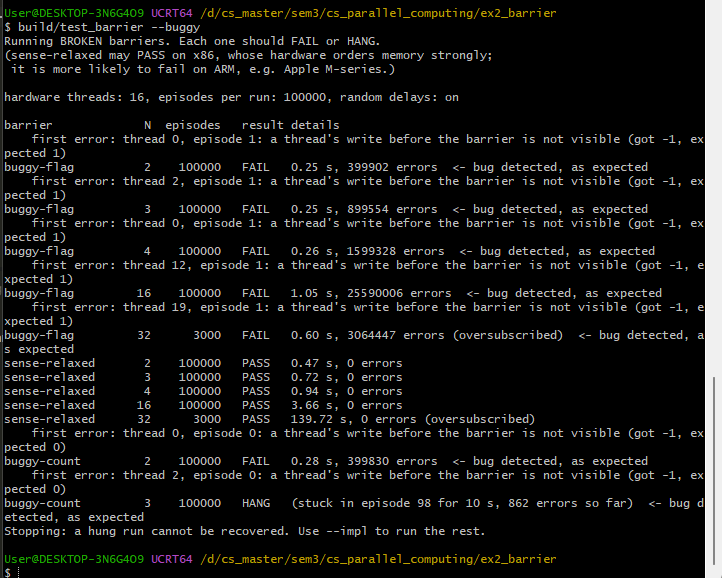
\includegraphics[width=0.95\textwidth]{figures/ex2_buggy_run.png}
\caption{Output of \texttt{build/test\_barrier --buggy} on Platform 1.}
\label{fig:ex2-buggy}
\end{figure}

\begin{table}[H]
\centering
\caption{Mutation testing on Platform 1 ($E=\num{100000}$ episodes, $3000$
for $N=32$).}
\label{tab:ex2-buggy}
\small
\begin{tabular}{lrlrl}
\toprule
\textbf{Barrier} & $N$ & \textbf{Result} & \textbf{Violations} & \textbf{Interpretation} \\
\midrule
\texttt{buggy-flag}    & 2  & FAIL & \num{399902}   & bug detected \\
\texttt{buggy-flag}    & 3  & FAIL & \num{899554}   & bug detected \\
\texttt{buggy-flag}    & 4  & FAIL & \num{1599328}  & bug detected \\
\texttt{buggy-flag}    & 16 & FAIL & \num{25590006} & bug detected \\
\texttt{buggy-flag}    & 32 & FAIL & \num{3064447}  & bug detected \\
\midrule
\texttt{sense-relaxed} & 2, 3, 4, 16, 32 & PASS & 0 & masked by x86-TSO (see text) \\
\midrule
\texttt{buggy-count}   & 2  & FAIL & \num{399830}   & bug detected \\
\texttt{buggy-count}   & 3  & HANG & 862 (stuck in episode 98) & bug detected \\
\bottomrule
\end{tabular}
\end{table}

\paragraph{\texttt{buggy-flag}.} The first violation is always reported in
\emph{episode 1}: a thread sees a slot still holding $-1$ instead of $1$.
This is exactly what the analysis of Attempt~2 predicts: episode $0$ works,
and since the flag is never re-armed, every later episode lets threads pass
straight through. The number of violations confirms it: with $N$ threads,
each thread performs $N$ slot checks per episode, so an always-failing
barrier produces about $N \cdot N \cdot E$ violations of (I1). For $N=2$
this is $2\cdot 2\cdot 10^5 = \num{400000}$, against \num{399902} measured;
for $N=16$ it is $\num{25600000}$, against \num{25590006} measured.
Essentially every check fails in every episode after the first.

\paragraph{\texttt{buggy-count}.} Both flaws of Attempt~1 show up. With
$N=2$, the barrier violates (I1) from episode $0$, in almost every check
(\num{399830} of $\approx\num{400000}$). The first arriving thread
increments \texttt{count} from $0$ to $1 = N-1$, so its own spin condition
is already true and it leaves before the second thread has arrived. This
is the early-departure bug described in Section~\ref{sec:ex2-naive}. With
$N=3$, the lost wake-up predicted by the lecture occurs as well: in
episode 98, a waiter misses the short window in which \texttt{count}
equals $N-1$, and the threads spin forever. The watchdog detects this
after \SI{10}{\second}. Since a hung run cannot be recovered, the remaining
configurations are not executed; this is expected.

\paragraph{\texttt{sense-relaxed}: a correct result that teaches a lesson.}
The relaxed variant is wrong according to the C++ memory model, yet it
passes all tests on Platform~1. The reason is the x86 memory model,
\emph{Total Store Order} (TSO)~\cite{sorin2020}: the hardware only allows
a store to be reordered after a later load (W$\to$R). Loads are not
reordered with other loads, and stores are not reordered with other stores,
and every x86 \texttt{LOCK}-prefixed RMW (such as \texttt{LOCK XADD} for
\texttt{fetch\_add}) is a full fence regardless of the requested C++ order.
The hardware therefore provides the acquire/release ordering ``for free'',
and as long as the compiler does not reorder the code, the bug stays
invisible. On processors with a weaker memory model, such as ARM (e.g.\
Apple M-series), stores and loads can be reordered, and (I1) is expected
to fail. The lesson is that \textbf{passing tests on x86 does not prove that
the memory orderings are correct}. The orderings in our implementation are
justified by the proof in Section~\ref{sec:ex2-proof}, not by the tests
alone.
% TODO (optional): if a group member owns an ARM machine (Apple M1/M2/M3),
% run `build/test_barrier --buggy --impl sense-relaxed` there and add the result.

% ---------------------------------------------------------------------
\subsection{Performance Results}
\label{sec:ex2-perf}

\subsubsection{Raw results on Platform 1}

Table~\ref{tab:ex2-perf} gives the median throughput (with minimum and
maximum over $R=5$ repetitions) and the corresponding median latency per
episode. Figure~\ref{fig:ex2-throughput} plots the throughput on a
logarithmic scale.

\begin{table}[H]
\centering
\caption{Barrier throughput on Platform 1 (episodes per second, median of 5
runs, with [min, max]), and median latency per episode.}
\label{tab:ex2-perf}
\scriptsize
\setlength{\tabcolsep}{3pt}
\begin{tabular}{l r r r r r}
\toprule
\textbf{Barrier} & $N=1$ & $N=2$ & $N=4$ & $N=8$ & $N=16$ \\
\midrule
\multicolumn{6}{l}{\emph{Throughput (episodes/s): median [min, max]}} \\
\texttt{sense-spin}      & 134.0\,M [117.4, 142.9] & 20.86\,M [19.79, 22.49] & 4.50\,M [4.12, 5.66] & 2.86\,M [2.59, 3.33] & 1.69\,M [1.54, 1.77] \\
\texttt{sense-backoff}   & 157.3\,M [156.0, 157.3] & 10.65\,M [10.43, 10.67] & 4.37\,M [4.20, 4.45] & 2.64\,M [2.48, 2.82] & 1.52\,M [1.46, 1.57] \\
\texttt{sense-yield}     & 157.3\,M [156.6, 157.3] & 20.90\,M [20.18, 20.91] & 4.36\,M [4.23, 4.61] & 2.91\,M [2.81, 3.13] & 0.17\,M [0.14, 0.18] \\
\texttt{sense-seqcst}    & 77.0\,M [76.5, 77.2]    & 15.82\,M [14.99, 17.71] & 4.45\,M [4.28, 4.74] & 2.70\,M [2.27, 2.79] & 1.29\,M [0.25, 1.40] \\
\texttt{std-barrier}     & 42.1\,M [42.0, 42.3]    & 478\,k [281, 887]       & 50.5\,k [41.0, 55.9] & 18.4\,k [18.0, 19.8] & 10.5\,k [10.3, 10.5] \\
\texttt{pthread-barrier} & 20.8\,M [20.3, 20.9]    & 208\,k [205, 213]       & 117\,k [115, 122]    & 58.5\,k [56.5, 59.4] & 34.9\,k [34.0, 35.0] \\
\texttt{openmp}          & ($\approx$100\,M)$^{\dagger}$ & 72.9\,k [71.1, 73.3] & 36.5\,k [36.2, 37.0] & 18.4\,k [18.3, 18.4] & 9.5\,k [9.5, 9.5] \\
\midrule
\multicolumn{6}{l}{\emph{Latency per episode (median)}} \\
\texttt{sense-spin}      & 7.5 ns  & 47.9 ns  & 222 ns  & 350 ns  & 593 ns \\
\texttt{sense-backoff}   & 6.4 ns  & 93.9 ns  & 229 ns  & 379 ns  & 657 ns \\
\texttt{sense-yield}     & 6.4 ns  & 47.8 ns  & 229 ns  & 344 ns  & 5.83 \textmu s \\
\texttt{sense-seqcst}    & 13.0 ns & 63.2 ns  & 225 ns  & 371 ns  & 776 ns \\
\texttt{std-barrier}     & 23.7 ns & 2.09 \textmu s & 19.8 \textmu s & 54.2 \textmu s & 95.7 \textmu s \\
\texttt{pthread-barrier} & 48.0 ns & 4.80 \textmu s & 8.53 \textmu s & 17.1 \textmu s & 28.7 \textmu s \\
\texttt{openmp}          & ---$^{\dagger}$ & 13.7 \textmu s & 27.4 \textmu s & 54.4 \textmu s & 105.5 \textmu s \\
\bottomrule
\end{tabular}

\vspace{2pt}
\raggedright\footnotesize $^{\dagger}$\,For $N=1$, the OpenMP run lasts only
1--2\,ms and \texttt{omp\_get\_wtime()} has a resolution of 1\,ms on this
platform, so the value is not reliable (individual runs show either 50\,M
or 100\,M episodes/s). It is excluded from the plots.
\end{table}

\begin{figure}[H]
\centering
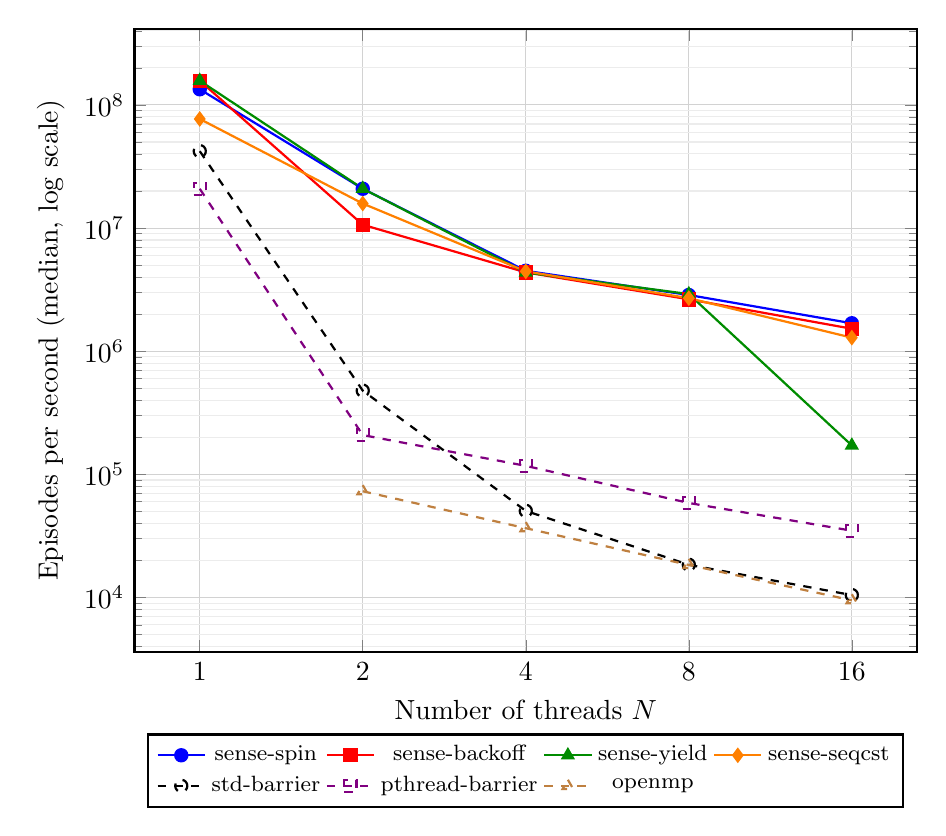
\begin{tikzpicture}
\begin{axis}[
    width=0.95\textwidth, height=9.5cm,
    xmode=log, log basis x=2, ymode=log,
    xtick={1,2,4,8,16}, xticklabels={1,2,4,8,16},
    xlabel={Number of threads $N$},
    ylabel={Episodes per second (median, log scale)},
    grid=both, minor grid style={gray!15}, major grid style={gray!35},
    legend style={at={(0.5,-0.13)}, anchor=north, font=\footnotesize},
    legend columns=4,
    mark size=2.2pt, thick,
]
\addplot[blue, mark=*] coordinates {(1,134048257) (2,20859408) (4,4497900) (8,2861165) (16,1686508)};
\addlegendentry{sense-spin}
\addplot[red, mark=square*] coordinates {(1,157282164) (2,10645659) (4,4368892) (8,2639177) (16,1522309)};
\addlegendentry{sense-backoff}
\addplot[green!55!black, mark=triangle*] coordinates {(1,157282164) (2,20899952) (4,4359103) (8,2911293) (16,171654)};
\addlegendentry{sense-yield}
\addplot[orange, mark=diamond*] coordinates {(1,76976368) (2,15822034) (4,4452875) (8,2696268) (16,1288092)};
\addlegendentry{sense-seqcst}
\addplot[black, dashed, mark=o] coordinates {(1,42131873) (2,478352) (4,50490) (8,18442) (16,10452)};
\addlegendentry{std-barrier}
\addplot[violet, dashed, mark=square] coordinates {(1,20835504) (2,208420) (4,117200) (8,58527) (16,34854)};
\addlegendentry{pthread-barrier}
\addplot[brown, dashed, mark=triangle] coordinates {(2,72886) (4,36523) (8,18366) (16,9482)};
\addlegendentry{openmp}
\end{axis}
\end{tikzpicture}
\caption{Barrier throughput versus number of threads on Platform 1 (higher
is better). Solid lines: our sense-reversing barrier variants. Dashed
lines: library barriers.}
\label{fig:ex2-throughput}
\end{figure}

\subsubsection{Comparison with existing barriers}

Figure~\ref{fig:ex2-speedup} shows how many times faster \texttt{sense-spin}
is than each library barrier.

\begin{figure}[H]
\centering
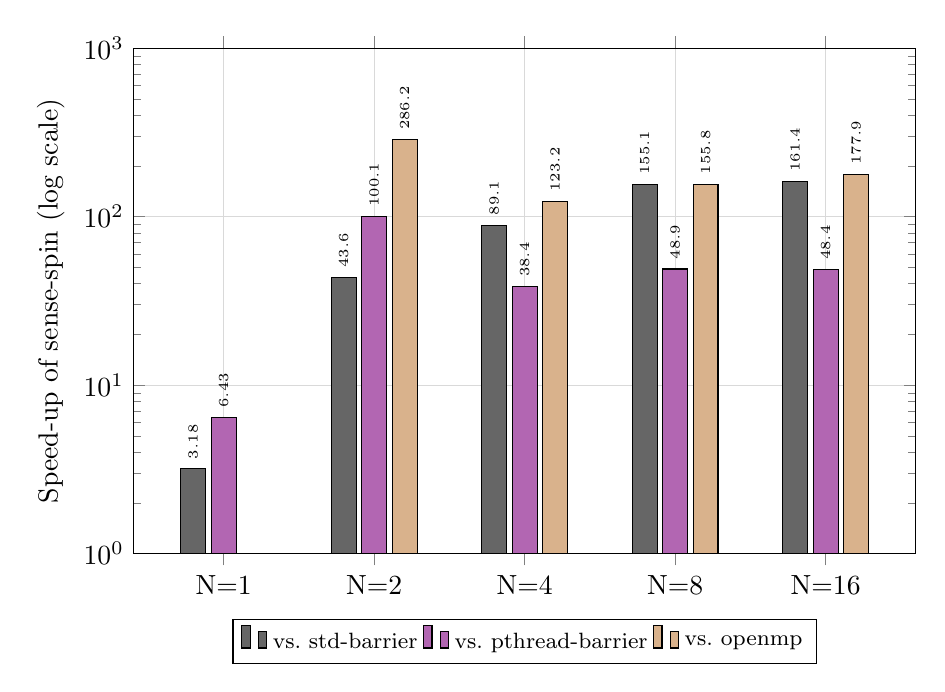
\begin{tikzpicture}
\begin{axis}[
    width=0.95\textwidth, height=8cm,
    ybar, bar width=9pt,
    ymode=log, log origin=infty,
    ymin=1, ymax=1000,
    symbolic x coords={N=1,N=2,N=4,N=8,N=16},
    xtick=data,
    ylabel={Speed-up of sense-spin (log scale)},
    legend style={at={(0.5,-0.13)}, anchor=north, font=\footnotesize},
    legend columns=3,
    nodes near coords, nodes near coords style={font=\tiny, rotate=90, anchor=west},
    point meta=rawy,
    grid=major, major grid style={gray!30},
    enlarge x limits=0.15,
]
\addplot[fill=black!60] coordinates {(N=1,3.18) (N=2,43.6) (N=4,89.1) (N=8,155.1) (N=16,161.4)};
\addlegendentry{vs.\ std-barrier}
\addplot[fill=violet!60] coordinates {(N=1,6.43) (N=2,100.1) (N=4,38.4) (N=8,48.9) (N=16,48.4)};
\addlegendentry{vs.\ pthread-barrier}
\addplot[fill=brown!60] coordinates {(N=2,286.2) (N=4,123.2) (N=8,155.8) (N=16,177.9)};
\addlegendentry{vs.\ openmp}
\end{axis}
\end{tikzpicture}
\caption{Throughput of \texttt{sense-spin} divided by the throughput of each
library barrier on Platform 1 (median values).}
\label{fig:ex2-speedup}
\end{figure}

Our sense-reversing barrier is \textbf{38$\times$ to 286$\times$ faster}
than all library barriers whenever $N \geq 2$. At $N = 16$ it completes
1.69 million episodes per second (\SI{593}{\nano\second} per episode),
versus \num{34854} for the fastest library barrier, Pthreads
(\SI{28.7}{\micro\second}), \num{10452} for \texttt{std::barrier} and
\num{9482} for OpenMP. The difference is caused by the waiting strategy
rather than by the arrival algorithm:

\begin{itemize}
    \item Our barrier \textbf{busy-waits}. A waiting thread notices the
          release within one cache miss (tens of nanoseconds).
    \item The library barriers on this platform \textbf{block}: waiting
          threads sleep in the Windows kernel and must be woken up by the
          last arriver through a system call, followed by a context switch.
          Each wake-up costs microseconds, and is paid in every episode.
    \item For \texttt{pthread-barrier} and \texttt{openmp}, the latency per
          episode grows almost exactly linearly with $N$ (Pthreads:
          \SIrange{1.8}{2.4}{\micro\second} per thread; OpenMP: a constant
          \SIrange{6.6}{6.9}{\micro\second} per thread). This is
          consistent with the last thread waking up the sleeping threads
          one by one.
    \item \texttt{std::barrier} (libstdc++) spins briefly before blocking.
          This explains why it is the fastest library barrier at $N=2$
          (\num{478}\,k episodes/s), where the wait is often short enough to
          end during the spin, but also why its performance is very
          variable there ([\num{281}\,k, \num{887}\,k]). From $N=4$ on, the
          wait outlasts the spin phase and it falls behind Pthreads.
\end{itemize}

The comparison must be read with its trade-off in mind. Blocking barriers
free the processor while waiting, which matters when phases are long or
when there are more threads than cores. Our barrier burns 100\% of each
waiting core; that is the price of its low latency. This is exactly the
spin-versus-block trade-off discussed in the lecture.

\paragraph{\texttt{OMP\_WAIT\_POLICY} has no measurable effect.}
Table~\ref{tab:ex2-omp} compares the three OpenMP runs. The differences
are within the run-to-run variation ($<3\%$). Even with
\texttt{OMP\_WAIT\_POLICY=active}, which should make libgomp threads spin
instead of sleeping, the barrier is two orders of magnitude slower than our
spinning barrier. This suggests that the MinGW build of libgomp used here
waits through Windows kernel objects in all modes. We did not investigate
the libgomp source further; on Linux, where libgomp spins on futexes, we
would expect \texttt{active} to be much faster.

\begin{table}[H]
\centering
\caption{OpenMP barrier throughput (episodes/s, median of 5) under different
\texttt{OMP\_WAIT\_POLICY} settings, Platform 1.}
\label{tab:ex2-omp}
\small
\begin{tabular}{lrrrr}
\toprule
\texttt{OMP\_WAIT\_POLICY} & $N=2$ & $N=4$ & $N=8$ & $N=16$ \\
\midrule
(default) & \num{72886} & \num{36523} & \num{18366} & \num{9482} \\
\texttt{active}  & \num{72254} & \num{37106} & \num{18416} & \num{9527} \\
\texttt{passive} & \num{71174} & \num{37622} & \num{18238} & \num{9571} \\
\bottomrule
\end{tabular}
\end{table}

\subsubsection{Scalability of the sense-reversing barrier}

Figure~\ref{fig:ex2-latency} plots the latency per episode of the
sense-reversing variants on a linear scale, and Table~\ref{tab:ex2-arrival}
divides it by $N$ to obtain the \emph{cost per arrival}.

\begin{figure}[H]
\centering
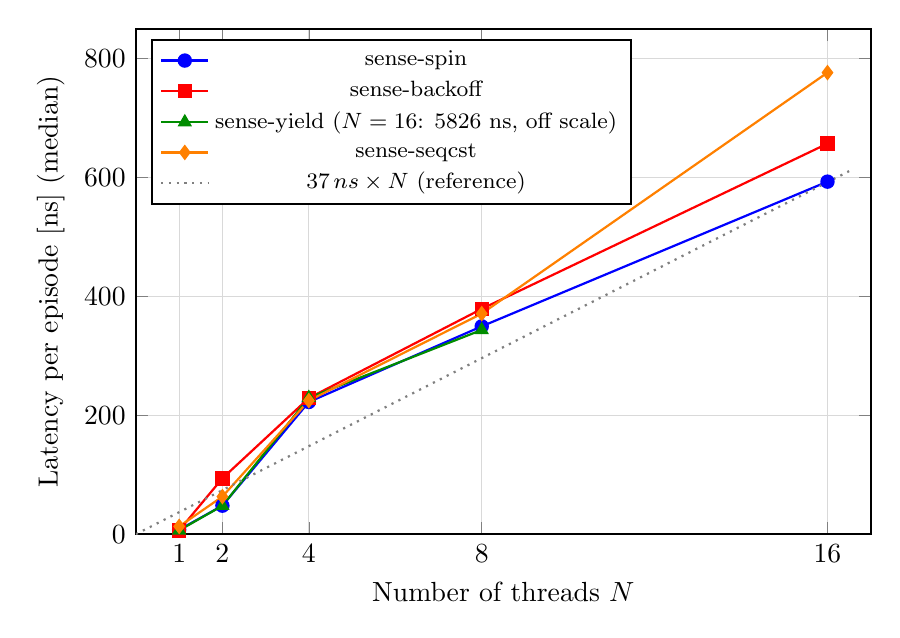
\begin{tikzpicture}
\begin{axis}[
    width=0.9\textwidth, height=8cm,
    xlabel={Number of threads $N$}, ylabel={Latency per episode [ns] (median)},
    xtick={1,2,4,8,16}, xmin=0, xmax=17, ymin=0, ymax=850,
    grid=major, major grid style={gray!30},
    legend style={at={(0.02,0.98)}, anchor=north west, font=\footnotesize},
    mark size=2.2pt, thick,
]
\addplot[blue, mark=*] coordinates {(1,7.5) (2,47.9) (4,222.3) (8,349.5) (16,592.9)};
\addlegendentry{sense-spin}
\addplot[red, mark=square*] coordinates {(1,6.4) (2,93.9) (4,228.9) (8,378.9) (16,656.9)};
\addlegendentry{sense-backoff}
\addplot[green!55!black, mark=triangle*] coordinates {(1,6.4) (2,47.8) (4,229.4) (8,343.5)};
\addlegendentry{sense-yield ($N=16$: 5826 ns, off scale)}
\addplot[orange, mark=diamond*] coordinates {(1,13.0) (2,63.2) (4,224.6) (8,370.9) (16,776.3)};
\addlegendentry{sense-seqcst}
\addplot[gray, dotted, domain=0:16.5, samples=2] {37*x};
\addlegendentry{$37\,\text{ns} \times N$ (reference)}
\end{axis}
\end{tikzpicture}
\caption{Latency per episode of the sense-reversing barrier variants on
Platform 1 (lower is better). The dotted line is a linear model
$37\,\text{ns} \cdot N$.}
\label{fig:ex2-latency}
\end{figure}

\begin{table}[H]
\centering
\caption{Median cost per arrival (latency per episode divided by $N$) on
Platform 1, in nanoseconds.}
\label{tab:ex2-arrival}
\small
\begin{tabular}{lrrrrr}
\toprule
\textbf{Barrier} & $N=1$ & $N=2$ & $N=4$ & $N=8$ & $N=16$ \\
\midrule
\texttt{sense-spin}    & 7.5  & 24.0 & 55.6 & 43.7 & 37.1 \\
\texttt{sense-backoff} & 6.4  & 47.0 & 57.2 & 47.4 & 41.1 \\
\texttt{sense-yield}   & 6.4  & 23.9 & 57.4 & 42.9 & 364.1 \\
\texttt{sense-seqcst}  & 13.0 & 31.6 & 56.1 & 46.4 & 48.5 \\
\bottomrule
\end{tabular}
\end{table}

\paragraph{The barrier does not scale; it degrades linearly.}
Throughput drops from 20.9\,M episodes/s at $N=2$ to 1.69\,M at $N=16$
(a factor of $12.4$ for an $8\times$ increase in $N$). The latency per
episode follows the linear model of Section~\ref{sec:ex2-costmodel}: from
$N=4$ onwards, the cost per arrival stays in a narrow band of about
\SIrange{37}{57}{\nano\second}. This is the typical cost of moving a
modified cache line from one core to another through the shared L3 cache,
i.e.\ $t_{\text{transfer}}$. The $N$ fetch-and-increment operations on
\texttt{count} are serialized, because the cache line can be exclusively
owned by only one core at a time, so they cannot be overlapped. Adding
threads therefore \emph{adds} time to every episode, and the centralized
sense-reversing barrier is inherently non-scalable.

\paragraph{Why the cost per arrival is not perfectly constant.}
\begin{itemize}
    \item $N=1$ (\SIrange{6}{13}{\nano\second}): no other core is involved.
          The cost is one uncontended \texttt{LOCK XADD} plus two stores
          hitting the local L1 cache.
    \item $N=2$ (\SI{24}{\nano\second} per arrival): the two threads run on
          different cores, but only one line transfer per arrival is
          needed. The operating system probably places both threads on
          P-cores.
    \item $N=4$ (\SI{56}{\nano\second}): the highest per-arrival cost.
          A likely cause is placement: with few threads the scheduler
          spreads them over distinct physical cores, so every transfer
          crosses the ring interconnect.
    \item $N=8$ and $N=16$ (\SIrange{37}{44}{\nano\second}): as more threads
          are added, some pairs run on \emph{sibling hyper-threads} of the
          same P-core, or on E-cores of the same cluster. Those pairs share
          an L1/L2 cache, so some transfers are cheaper. We did not pin
          threads, so this interpretation is plausible but not verified
          (see Section~\ref{sec:ex2-threats}).
\end{itemize}

\subsubsection{Effect of exponential backoff}

Exponential backoff \textbf{does not improve} the sense-reversing barrier
on Platform~1. It is $2\times$ slower at $N=2$ (10.6\,M versus 20.9\,M
episodes/s) and 3--10\% slower at $N \geq 4$. This is not an implementation
flaw; it follows from the structure of the algorithm:

\begin{itemize}
    \item Backoff reduces contention in \emph{retry loops}, where many
          threads repeatedly attempt a failing RMW on the same location
          (TAS/CAS locks, Exercise~1). Each failed attempt generates
          coherence traffic, and spacing attempts out reduces it.
    \item In the sense-reversing barrier, the contended RMW (the FAI on
          \texttt{count}) is executed exactly \emph{once} per thread per
          episode and never fails or retries. The spinning, which is what
          we back off, is a read-only loop on a cached copy of
          \texttt{sense}, which generates no traffic at all. Backoff
          therefore has nothing to reduce.
    \item Backoff does have a cost: a thread that has backed off for $k$
          rounds notices the release up to $2^{k}$ \texttt{PAUSE}s late. At
          $N=2$ an episode lasts only about \SI{48}{\nano\second}, so even a
          few extra \texttt{PAUSE}s (each tens of cycles) double the
          latency. At larger $N$ the episode is longer and the relative
          penalty shrinks, but it never turns into a gain.
\end{itemize}

Backoff would be useful in a variant that \emph{does} retry, such as a
barrier whose arrival is implemented with a CAS loop, or on a non-coherent
or very large NUMA system where even spinning on a remote line is
expensive.

\subsubsection{Effect of yielding}

\texttt{sense-yield} behaves exactly like \texttt{sense-spin} for $N \leq 8$:
episodes are short, so a waiter almost never exhausts its 128 spins and
never calls \texttt{yield}. At $N=16$, however, its throughput collapses by
a factor of $10$ (\num{171654} versus \num{1686508} episodes/s, about
\SI{5.8}{\micro\second} per episode). Our explanation:

\begin{itemize}
    \item With $N = H = 16$, all logical processors are busy, and some
          threads run on the slower E-cores. Occasionally an episode takes
          longer than the 128-spin budget, so waiters start calling
          \texttt{std::this\_thread::yield()} (\texttt{SwitchToThread} on
          Windows).
    \item Each call is a system call costing on the order of a
          microsecond. A thread inside the kernel cannot see the release, so
          it reacts late. Once threads are late, the next episodes are slow
          as well, and the slowdown feeds on itself.
\end{itemize}

The other side of the same trade-off appears in the correctness tests,
where many threads are descheduled (random delays, oversubscription with
$N=32$). In the oversubscribed test (Table~\ref{tab:ex2-test}),
\texttt{sense-yield} finished 3000 episodes in \SI{0.17}{\second}, while
\texttt{sense-backoff} needed \SI{127}{\second} for the same 3000 episodes
and \texttt{sense-spin} \SI{12.6}{\second} for only 300. The same pattern
appears at $N=16$ with random delays: \SI{3.4}{\second} for
\texttt{sense-yield}, against \SI{62}{\second} for \texttt{sense-backoff}
and \SI{500}{\second} for \texttt{sense-spin}. Spinning threads waste the
time slices that a preempted or delayed thread needs to make progress. \textbf{Yielding is harmful when
every thread has its own core, and essential when threads outnumber
cores.} A production barrier would use an adaptive policy, or a much larger
spin budget before yielding.

\subsubsection{Effect of memory ordering}

The sequentially consistent variant is \textbf{$1.7\times$ slower at $N=1$}
(\SI{13.0}{\nano\second} versus \SI{7.5}{\nano\second}). On x86, the RMW
(\texttt{LOCK XADD}) and the loads compile to the same instructions for
both orderings, so the difference comes from the two stores, which become
\texttt{XCHG} (an implicitly locked, fully fenced instruction) instead of
a plain \texttt{MOV}. For $N=2..8$ the gap shrinks to 0--32\%, because the
coherence traffic dominates the cost of an episode. At $N=16$ the median is
24\% lower, but this run also contains the largest outlier of the whole
study (one repetition at \num{248374} episodes/s, caused by OS
interference). The results support the choice of acquire/release
orderings: they are provably sufficient and never slower.

\subsubsection{Variability}

The variation between repetitions is small for the spinning barriers
($\pm 10\%$ around the median in most configurations). The largest
spreads are:
\begin{itemize}
    \item \texttt{std-barrier} at $N=2$ (\num{281}\,k--\num{887}\,k): the
          spin-then-block strategy is sensitive to whether the partner
          thread arrives before or after the spin phase ends;
    \item single outliers in \texttt{sense-seqcst} ($N=16$) and
          \texttt{sense-spin} ($N=4$), consistent with occasional OS
          interference when no processor is idle.
\end{itemize}
Reporting the median of five runs makes the conclusions insensitive to
these outliers.

% ---------------------------------------------------------------------
\subsection{Results on Other Platforms}
\label{sec:ex2-other}

% TODO: fill in once Platforms 2 and 3 have been measured.
% For each platform:
%   1. ./build.sh && build/test_barrier          -> add PASS/FAIL row(s)
%   2. build/bench_barrier > results_laptopX.csv
%   3. add the median values to a table and a throughput plot as in
%      Table~\ref{tab:ex2-perf} and Figure~\ref{fig:ex2-throughput}
\textcolor{red}{[TODO: results of Platforms 2 and 3. The assignment requires
at least as many platforms as group members.]}

% ---------------------------------------------------------------------
\subsection{Discussion}
\label{sec:ex2-discussion}

\subsubsection{Summary of findings}

\begin{enumerate}
    \item The sense-reversing barrier is \textbf{correct}. Our argument
          shows safety, liveness, reusability and the required
          happens-before ordering. The test harness confirms this on 30
          configurations and is shown to catch both incorrect barriers from
          the lecture.
    \item It is \textbf{very fast for small thread counts}: about
          \SI{48}{\nano\second} per episode for two threads and
          \SI{0.6}{\micro\second} for 16 threads, i.e.\ 38--286$\times$
          faster than the \texttt{std::barrier}, Pthreads and OpenMP
          barriers available on Windows/MinGW, all of which block in the
          kernel.
    \item It is \textbf{not scalable}: the latency per episode grows
          linearly with $N$ (about \SIrange{40}{55}{\nano\second} per
          thread), because all arrivals are serialized on one cache line.
          For large $N$, tree or dissemination barriers are needed.
    \item \textbf{Exponential backoff does not help}, because the barrier's
          contended RMW never retries and its spinning causes no traffic.
          \textbf{Yielding} is harmful when each thread has its own core
          but essential under oversubscription.
    \item \textbf{Acquire/release orderings} are sufficient and slightly
          faster than sequential consistency. Fully relaxed orderings are
          incorrect, even though x86 hides the error.
\end{enumerate}

\subsubsection{Threats to validity}
\label{sec:ex2-threats}

\begin{itemize}
    \item \textbf{No thread pinning.} Threads were placed by the Windows
          scheduler. On a hybrid CPU, placement (P-core vs.\ E-core,
          sibling hyper-threads) affects the cost of cache line transfers.
          Pinning (\texttt{SetThreadAffinityMask}) would make the
          per-arrival analysis more precise.
    \item \textbf{Power plan.} Measurements were taken with the
          ``Balanced'' power plan, which allows frequency scaling. Warm-up
          episodes reduce, but do not eliminate, this effect.
    \item \textbf{Timer resolution of OpenMP.} \texttt{omp\_get\_wtime()}
          has a resolution of \SI{1}{\milli\second} on this platform, so the
          OpenMP value for $N=1$ is unreliable. All other OpenMP runs last
          more than \SI{1}{\second}, where the error is below 0.1\%.
    \item \textbf{Library implementations are platform specific.} The poor
          performance of the library barriers reflects their MinGW/Windows
          implementations (libstdc++, winpthreads, libgomp). On Linux, the
          same libraries use futexes and are expected to be considerably
          faster, so the measured speed-ups should not be generalised.
    \item \textbf{Testing is not proof.} The x86-TSO result for
          \texttt{sense-relaxed} shows that the tests cannot reveal every
          memory-ordering bug on a strongly ordered machine.
\end{itemize}

\subsubsection{Possible extensions}

\begin{itemize}
    \item Implement the dissemination and the tree barriers from the
          lecture, and compare their scalability with the centralized
          barrier.
    \item Measure with a small, variable amount of work between barriers,
          to quantify how load imbalance interacts with the waiting
          policies.
    \item Replace the fixed spin budget of \texttt{sense-yield} with an
          adaptive one, or use C++20 \texttt{std::atomic::wait} for a hybrid
          spin-then-block barrier.
\end{itemize}

\subsection{How to Reproduce}
\label{sec:ex2-reproduce}

\begin{lstlisting}[numbers=none,language=bash]
cd ex2_barrier
./build.sh                                   # GCC >= 11 with OpenMP
build/test_barrier                           # correctness, all barriers
build/test_barrier --buggy                   # mutation testing
build/bench_barrier > results_<machine>.csv  # performance
OMP_WAIT_POLICY=active  build/bench_barrier --impl openmp > omp_active.csv
OMP_WAIT_POLICY=passive build/bench_barrier --impl openmp > omp_passive.csv
python plot_results.py results_<machine>.csv
\end{lstlisting}
